\subsection{Problem discussion, in the Sokoban domain}
Sokoban is a game originating from Japan. The essence of the game is to push jewels around in a room containing obstacles, in a manner that will enable the player to place all the jewels on so called goals in the room. See figure \ref{fig:sokohero} for a screenshot of a sokoban game.
Sokoban is an interesting game to study in the domain of Artificial Intelligence, because it presents a so called NP-complete problem, meaning in this case that it is often fairly easy for humans to solve such puzzles in a manner of minutes, but very difficult to develop an efficient algorithm able to do the same. This is due to the fact that NP-complete problems spawn huge search trees and branch factors.

\subsubsection{The rules of the game}
The rules of the game are simple. The game is best described as consisting of squares, each having an (x, y) coordinate. A game consists of the following squares:
\begin{itemize}
\item One 'Man' square, representing the player. The 'Man' square can move around.
\item One or more 'Jewel' squares representing objects that have to be pushed onto 'Goal' squares by the player.
\item One or more 'Goal' squares. There are always the same amount of 'goal' squares as 'Jewel' squares.
\item One or more 'Wall' representing impenetrable boundaries which can not be passed by neither 'Man' nor 'Jewel' squares.
\item One or more 'Empty' squares representing space where the player/'Man' square is able to move. 
\end{itemize}

\begin{figure}[ht]
\centering
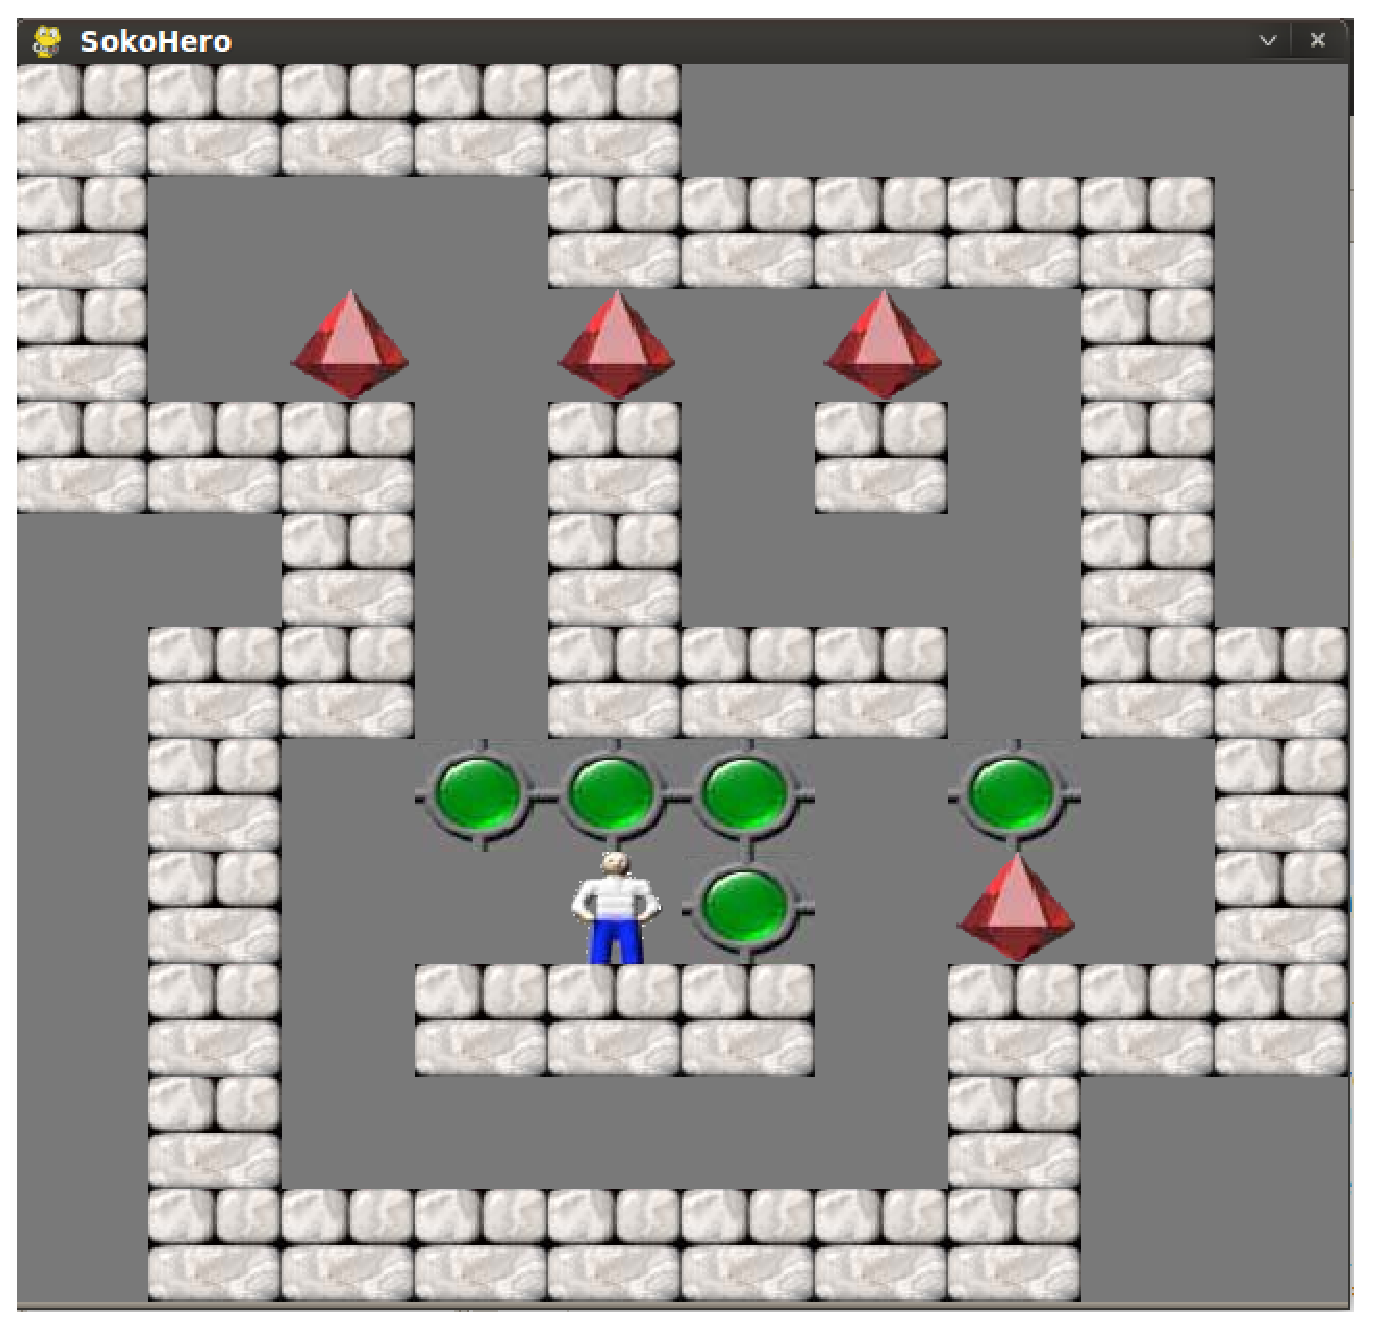
\includegraphics[scale=0.25]{images/sokohero.eps}
\caption{A screenshot of a sokoban game}
\label{fig:sokohero}
\end{figure}


As stated previously the purpose of the game is for the player to push 'Jewel' squares onto 'Goal' squares. That the player is only able to push jewels signifies that if a jewel is at position (x, y), and the player is at position (x - 1, y) then the player will be able to move the jewel to position (x + 1, y) if (x + 1, y) is occupied by an 'Empty' or a 'Goal' square. The same logic applies for other directions.
 
\subsubsection{Challenges faced when solving Sokoban algorithmically}
Given the fact that the player can on average move up, down, left and right, we see that the problem presents a so called branching factor of 4. If an algorithm is able to solve the puzzle in 100 moves, the complexity becomes 4$^{100}$ . 
This enormous complexity, illustrates the need for some sort of heuristics or pruning of the search tree, if the problem is to be solved in an acceptable time frame.
Deadlocks are one of the main challenges faced when trying to solve the Sokoban puzzle. A deadlock is best described as a situation where a jewel is pushed into a position that eliminates the possibility of solving the puzzle, for instance pushing a jewel into a corner. 

\subsubsection{Algorithmic approach}
The general approach taken to solve the sokoban problem, is creating a search tree where every node in the tree is a state of the game. The goal is then to traverse the tree to find the state where all of the coordinates of the jewels match the coordinates of all the goals.\\
The general algorithmic search can described as:

\begin{lstlisting}[language=Ruby, frame=single, basicstyle=\small, caption={Deadlock detection pseudo code}, label={code:sokoalgo}]
if not problem solved:
	get next state in search tree
	if state not goal state:
		for each jewel in state do:
			for every direction in which jewel can move one square do:
				if resulting state would be valid and resulting state not duplicate of a previous state:
					if robot can get to the position to push the jewel in the desired direction:
						create new state				
						move jewel to new position
						move robot to previous jewel position
						calculate state score
						add state to search tree	
\end{lstlisting}

As can be seen from the pseudo code, the problem solving can logically be divided into two separate subproblems, the first one being the movement of the jewels, henceforth known as the jewel problem, and the second being the path finding from the robot to the jewel that has to be moved, henceforth known as the path finding problem. 
The search approach best suited for the solving of these two distinct areas might not be the same, and therefore each subproblem is considered separately, and the solution implemented will treat the subproblems as two seperate search trees. 